%------------------------------------
% Document Preamble
%------------------------------------
\documentclass[12pt, a4paper]{article}
\setlength{\oddsidemargin}{0.5cm}
\setlength{\evensidemargin}{0.5cm}
\setlength{\topmargin}{-1.6cm}
\setlength{\leftmargin}{0.5cm}
\setlength{\rightmargin}{0.5cm}
\setlength{\textheight}{24.00cm} 
\setlength{\textwidth}{15.00cm}
\parindent 0pt
\parskip 5pt
\pagestyle{plain}

%------------------------------------
% Imported packages
%------------------------------------
\usepackage{graphicx}
\usepackage{lscape}
\usepackage{rotating}
\usepackage{siunitx}
\usepackage{wrapfig}
\usepackage[hyphens]{url}

%------------------------------------
% Graphics path specification
%------------------------------------
\graphicspath{{./fig/}}

%------------------------------------
% Title block
%------------------------------------
\title{ENG720: Research Proposal}
\author{}
\date{}

\newcommand{\namelistlabel}[1]{\mbox{#1}\hfil}
\newenvironment{namelist}[1]{%1
\begin{list}{}
    {
        \let\makelabel\namelistlabel
        \settowidth{\labelwidth}{#1}
        \setlength{\leftmargin}{1.1\labelwidth}
    }
  }{%1
\end{list}}

\begin{document}
\maketitle

\begin{namelist}{xxxxxxxxxxxx}
\item[{\bf Title:}]
	Automatic generation control of a two area power system using deep reinforcement learning
\item[{\bf Author:}]
	Shane Reynolds
\item[{\bf Supervisor:}]
	Charles Yeo \& TBC
\item[{\bf Degree:}]
	Bachelor of Engineering (Honours)
\end{namelist}


%------------------------------------
% Contents
%------------------------------------
\tableofcontents
\newpage

%------------------------------------
% Introduction and Background
%------------------------------------
\section{Introduction \& Background}
In 2018 there was approximately 261$\si{\tera\watt\hour}$ of power generation in the Australian electricity sector. Renewables contributed to 19\% of the total generation, increasing from 15\% in 2017 \cite{Gov202002}. This is a pattern which has followed on from 2016. Indeed, a trend of greater renewable energy penetration in the electricity generation market has emerged starting in approximately 2008, as shown in Figure 1.
\begin{figure}[h]
	\centering
	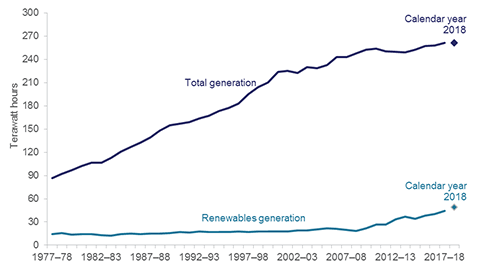
\includegraphics[height=7cm]{australian_generation_profile}
	\caption{text}
\end{figure}

One of the benefits of transitioning from thermal sources of generation to renewable sources is reduced greenhouse gas emissions (REFERENCE), however, this transition is not without its drawbacks. Increased reliance on renewable generation sources has introduced some challenges regarding power system stability. A recent example is the system failure resulting from an event cascade, triggered by cloud cover shadowing a solar array in Alice Springs. The system failure resulted in a blackout occurring in Alice Springs for approximately 8 hours (REFERENCE). The Entura report highlighted that poor control policies were one of the many factors contributing to the blackout. In this instance, a generator provisioned to ramp up in the event of cloud cover limiting solar array output was unable to be controlled (REFERENCE). Moreover, generators that were still under the control regime were issued operating set points above their rated capacity, which eventually resulted in thermal overload and subsequent tripping from the protection system.\\

One of the issues with currently employed control methods (using classical techniques) is that they can be brittle when faced with system changes, or scenarios which they were not designed for/ envisioned. A more robust controller would be one that can learn and adapt to a system, given some broad control objective. (NEED TO REPHRASE THIS ASPECT). This research proposes a Deep Reinforcement Learning agent for controlling the frequency of a power system with multiple generators, and multiple stochastic loads. Existing approaches currently employ classical engineering control methodologies.

\clearpage

\subsection{Power Systems and Frequency}
Interconnected power systems are comprised of power generating units and energy storage systems connected to transmission and distribution networks. Generated power is used to service load demand. A single line diagram of a power network can be seen in Figure 1. The left hand side of the diagram shows thermal generation units, such as coal and nuclear, in addition to renewable sources of generation, like wind and solar. The right hand side of the figure shows the distribution network and the consumers of generated energy: industry and households.
\begin{figure}[h]
	\centering
	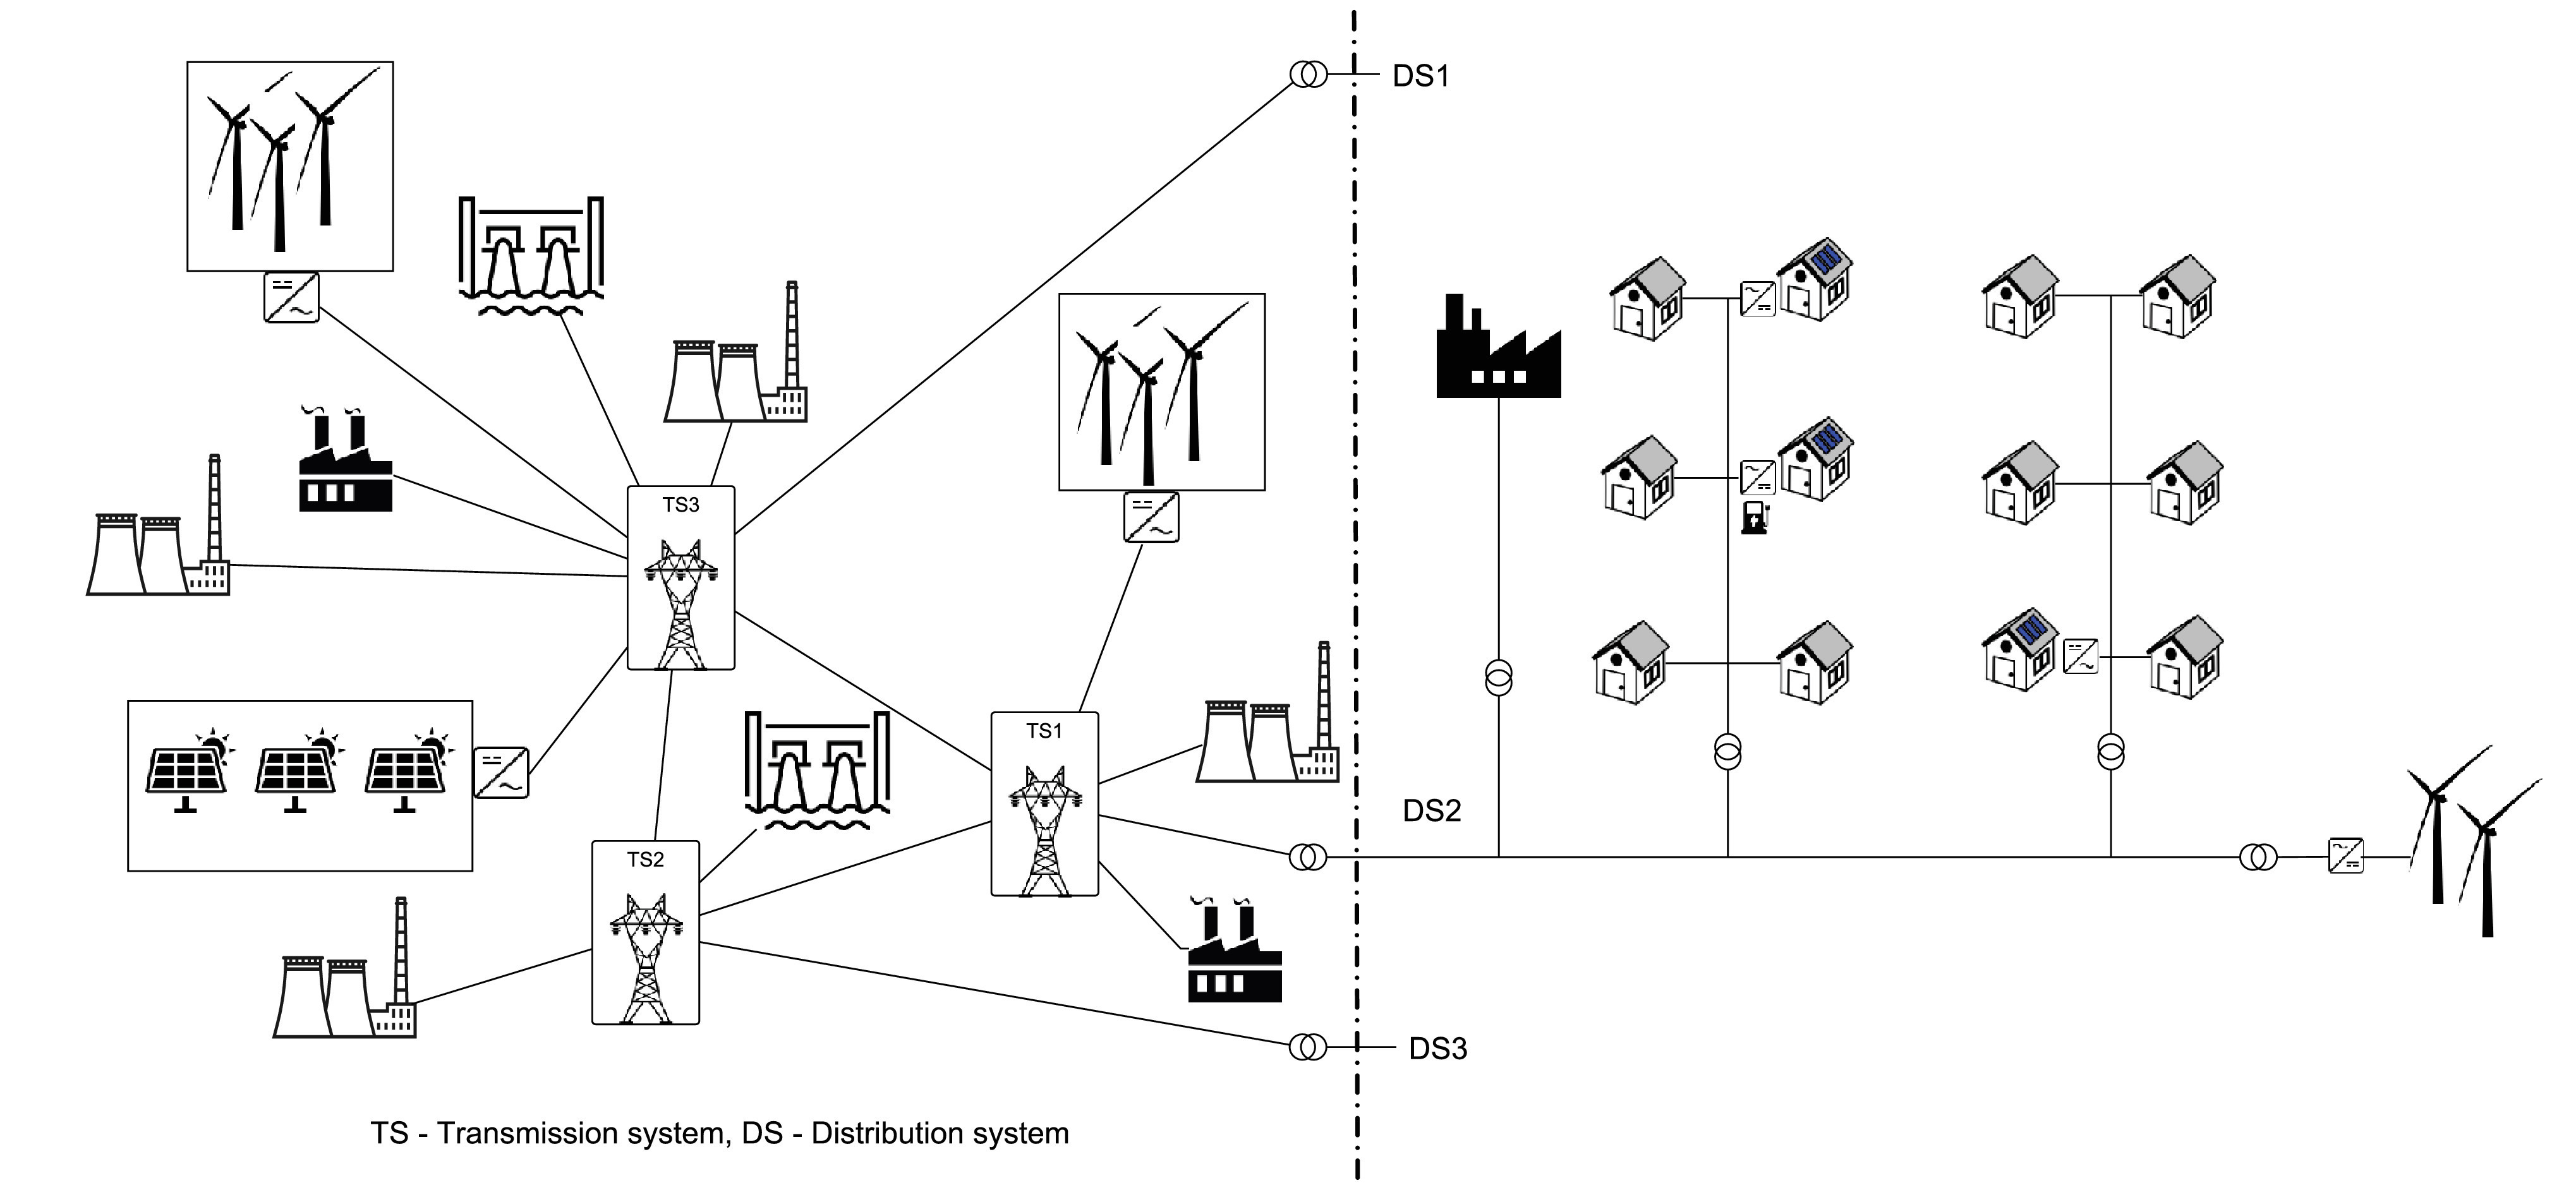
\includegraphics[scale=0.85]{power_system}
	\caption{A single line diagram of a typical power system taken from \cite{Glavic2019}. The image shows points of generation from thermal and renewable sources, and the subsequent supply of generated energy to meet load demand through the transmission and distribution network.}
\end{figure}

One of the key elements to successful operation of interconnected power systems is ensuring total load demand is matched with total generation, taking into account power losses involved with generation, transmission, and distribution \cite{Wood2013}. To understand why it is important to match generation with load demand it is useful to first consider the basic operation of a single thermal generator. 
\begin{figure}[h]
\centering
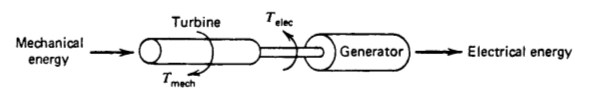
\includegraphics[height=1.4cm]{generation}
\caption{A thermal generation unit consists of a prime mover (turbine), and a synchronous machine. This image was taken from \cite{Wood2013}.}
\end{figure}

The essential elements of a thermal generator are a prime mover (turbine) and a synchronous machine, as depicted in Figure 2. The prime mover provides mechanical torque, $T_{mech}$, which drives the synchronous machine producing electrical energy. In response, the synchronous machine creates a torque which opposes $T_{mech}$, dependent on the size of the load demand from households and industry. This is referred to as electrical torque and is denoted as $T_{elec}$. If $\alpha$ represents angular velocity of the generator rotating mass, and $I$ is its moment of inertia, then by Newton's second law:
\begin{equation}
\sum T_i = I \alpha 
\end{equation}

Equation (1) shows that when $T_{mech}$ equals $T_{elec}$ the system will be in a steady state with zero angular acceleration, and a constant rotation at some angular velocity $\omega$. Now, if $T_{mech} > T_{elec}$, then the angular velocity $\omega$ of the system will increase as the system speeds up, resulting in a frequency increase in the system. Conversely, if $T_{mech} < T_{elec}$ then the angular velocity $\omega$ will decrease as the system slows down, resulting in a frequency decrease. What makes this situation interesting is that at any point in time the total electrical load demand will fluctuate stochastically, meaning that an uncontrolled system will have a continually changing frequency. Australia's electricity network is designed to operate at a frequency of 50$\si{\hertz}$. In the majority of network scenarios AEMO has a desired operating range for frequency which lies between 49.85$\si{\hertz}$ and 50.15$\si{\hertz}$ \cite{AEMO2012}. Similarly, the PWC Network Technical Code for the Northern Territory states that under normal operating conditions frequency should be maintained in the range 49.80$\si{\hertz}$ to 50.20$\si{\hertz}$ \cite{PWC2018}. Operation outside of specified ranges can cause damage to electrical equipment such as transformers or motors, which are designed to operate at specific frequencies \cite{Sen2014}. Network designers engineer protection schemes so that sustained frequency excursions outside of the allowed range will cause equipment to trip from the network \cite{AEMO201804}. Protection schemes tripping equipment from the network is undesirable since this can leave households and industry without power, resulting in economic loss. Further, if disconnections are uncontrolled then this can lead to a further loss of system stability \cite{AEMO201804}.

\begin{figure}[h]
	\centering
	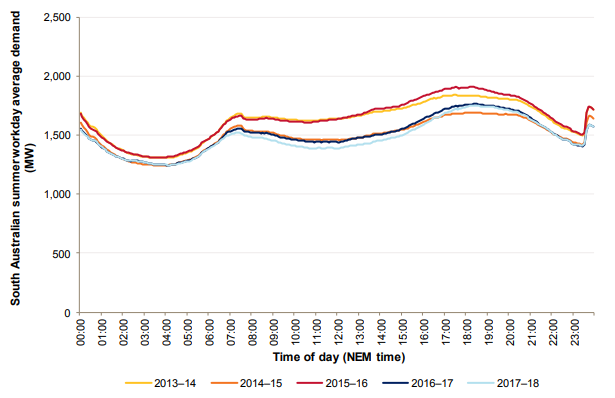
\includegraphics[height=7cm]{load_profile}
	\caption{Weekday energy demand profile in South Australia during summer \cite{AEMO2018}.}
\end{figure}

System controllers, such as the Australian Energy Market Operator (AEMO) and Power and Water Corporation (PWC), are therefore interested in being able to control the system to follow changes in load demand so that system frequency is maintained in the allowable range. Additionally, they are interested in control mechanisms to restore frequency excursions as a result of unexpected disturbances. System controllers can use historical data to forecast daily demand profiles with some reliability. A plot of average historical data, for the daily demand profile in South Australia during Summer, can be seen in Figure 3. This type of forecasting does not help when trying to predict the occurrence of random disturbances, however, it does provide a starting point for estimating required generation needed to meet demand. It is important to note that forecasting is not perfect. Inevitably mismatches in supply and demand will occur causing small imbalances between $T_{mech}$ and $T_{elec}$, resulting in a change to angular velocity $\omega$ and the network frequency \cite{Glover2012}. To perfectly match supply and demand, system controllers use generators referred to as regulating units \cite{Kothari2011}. A regulating unit is a generator that has capacity to increase or decrease mechanical torque $T_{mech}$ allowing the system controller to provide two functions: load following; and restoring the system to stable operating conditions in the event of a disturbance \cite{Grainger1994}. Using a regulating unit to load follow is referred to as the provision load following ancillary services \cite{AEMO202002}. Load following control adjusts regulating units slightly to match supply perfectly with a demand load profile, like that shown in Figure 3. Using a regulator to restore the system after a disturbance is referred to as providing spinning reserves \cite{AEMO202002}. When used in this fashion the regulating unit is not responsible for arresting frequency excursions, rather, it is used to restore the system back to the allowable frequency operating range after the frequency excursion has been arrested. An example of a frequency excursion, arrest, and subsequent restoration can be seen in Figure XXXX.

\begin{figure}[h]
\centering
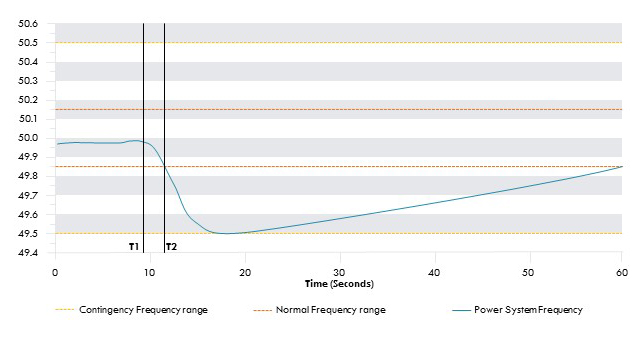
\includegraphics[height=8cm]{frequency_arrest}
\caption{A frequency disturbance occurs just before the 10 second mark, and regulating units ramp up their generation to first arrest the disturbance, and provide the subsequent correction, returning system frequency to 50$\si{\hertz}$.}
\end{figure}

AEMO and PWC do not require all generators on the network to act as regulating units since adequate frequency control can be achieved using a subset of the available generators.

\subsection{Load frequency control for a single area}
The power system model shown in Figure 1, on page 2, depicts total generation coming from many generation assets - this is complex to model. Researchers often find it useful to divide generation assets into sub-groups referred to as control areas \cite{Kothari2011}. A control area is defined as a subset of generators which are in close proximity to each other and constitute a coherent group that speed up and slow down together, maintaining their relative power angles \cite{Kothari2011}. The total network is therefore comprised of many interconnected control areas. An example of a series of interconnected control areas can be seen in Figure 5. Notice that for each area there is only a single load and a single generator. Typically, for each control area, researchers will aggregate many loads into a single load, and many generators into a single generator. This simplifies the model further \cite{Grainger1994}.
\begin{figure}[h]
	\centering
	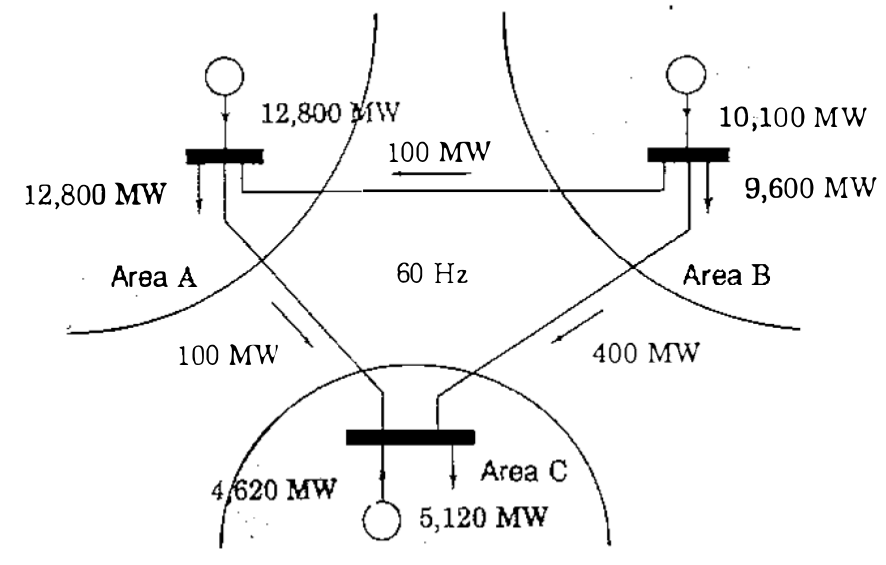
\includegraphics[height=8cm]{multiple_area_system}
	\caption{An example of three interconnected control areas in a 60$\si{\hertz}$ power system. The interconnections allow power to flow from one area to another, allowing generators to service loads from different areas. Each control area is consists of many generators and loads, but are modelled with a single generator and single load, respectively \cite{Grainger1994}.}
\end{figure}

The simplest power system to control is one that consists of a single control area, such as Area A in Figure 5. This power system has no interconnections to any other control area. It is comprised of consumer load demand, and a set of generators, some of which are acting as regulating units. As previously mentioned, for modelling simplicity, loads are aggregated to a single load, and generators are aggregated to a single generator. This classic, simple system is well understood and it is generally acknowledged that a governor feedback control regime can successfully perform frequency control of the system \cite{Wood2013, Grainger1994, Kothari2011}. Most introductory textbooks on power systems cover governor control of this system. Kothari (2011) provides a particularly well laid out approach to developing linear models for the turbine, generator load, and governor for the system - the full model can be seen in Figure 6 \cite{Kothari2011}. The leftmost block is a first-order linear model of the speed governor, the second block is a first-order model of the turbine, which the controller directly acts on. The final block is the generator load, which is also a first order system. The over all system model is a second order linear model, with a first order controller.

\begin{figure}[h]
\centering
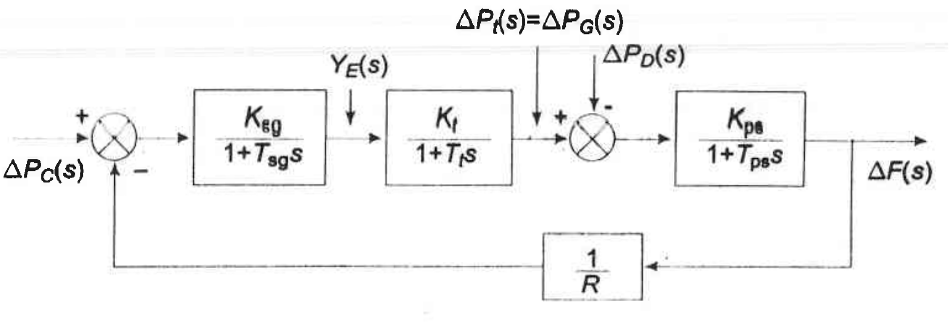
\includegraphics[height=5cm]{single_area_control}
\caption{A classical feed back control approach to a second order linear system. The second order system is comprised of a first order model for both the turbine, and generator load. The controller is modelled as a first order system \cite{Kothari2011}.}
\end{figure}


\subsection{Two-area load frequency control}
The system presented in Section 2.2 is useful to help understand the role of governors in controlling power system frequency, however, a single area model is too simple. In reality, power systems are comprised of many control areas connected through tie lines, which are typically transmission lines \cite{NPTEL202002}. Distinct control areas are often thought of as different participants in the generation market, or simply as different regions in which generation assets are based \cite{NPTEL202002}. The simplest model which includes tie lines is the two area power system \cite{Kothari2011}. 

\begin{figure}[h]
	\centering
	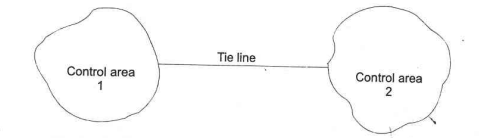
\includegraphics[height=3cm]{two_area_system}
	\caption{Two area power system is comprised of generators and load connected via a tie line. Power flows from one area to the other depending on economic contracts.}
\end{figure}

Two area power systems are well understood. Linear models have been developed, and classical control approaches analysed using governors on both

TALK ABOUT WHAT HAPPENS IF WE JUST LET THE SPEED GOVENORS DO THE JOB

TALK ABOUT HOW THIS MAY END UP VIOLATING ECONOMIC CONTRACTS THAT ARE IN PLACE

INTRODUCE AUTOMATIC GENERATION CONTROL AND THE ITS PRIMARY MOTIVATION

TALK ABOUT THIS LARGELY BEING A SOLVED PROBLEM

\subsection{Reinforcement learning}

TALK ABOUT THE HISTORY OF REINFORCEMENT LEARNING

TALK ABOUT APPLICATIONS IN THIS FIELD

\subsubsection{Markov Decision Process}
Reinforcement Learning (RL) is a branch of machine learning that is concerned with how agents make sequential decisions to maximise some notion of a cumulative reward. Suppose that a robotic agent exists in some environment which is comprised of many discrete states, $s \in S$, such that $S$ denotes the state space. At any discrete point in time the agent can take an action $a \in A$, where $A$ denotes the action space. When the agent takes an action in a given state, the agent receives some reward, denoted with $r \in R$, where $R$ is the reward set. If an agent is in a given state, $s$, and takes and action, $a$, this will transition the agent to a new state, $s'$, and yield reward, $r$, with some given probability - these are referred to as state transition probabilities. Transition probabilities are denoted as follows:
\begin{equation}
P(S_{t+1}=s', R_{t+1}=r \ | \ S_t = s, A_t = a)
\end{equation}

The set of parameters, outlined above, make up a framework referred to as a Markov Decision Process (MDP).

\subsubsection{Policy}
In order for the robot to act within the environment, it needs to have a policy. A policy, $\pi$, is defined as a mapping from states to actions, that is, a rule which determines what action the robot will take for a given state. A deterministic policy, $\pi (s)$, maps a single action to a single state. A stochastic policy, $\pi (a | s)$, defines a probability distribution over the actions for a given state.

\subsubsection{Return}
As the robotic agent takes actions at each discrete time step, it receives a reward. The cumulative sum of this reward is referred to as the return. The return is denoted, for $N$ discrete time steps, as:
\begin{equation}
G_t = r_t + r_{1+1} + r_{t+2} + \ldots + r_{N-1}
\end{equation}

Often it is convenient to make future rewards less important that more immediate rewards. This is by multiplying each reward in the sequence by a discount factor, $\gamma \in [0,1]$. Equation (XXXX) then becomes:
\begin{equation}
G_t = r_t + \gamma r_{1+1} + \gamma^2 r_{t+2} + \ldots + \gamma^{N-1} r_{N-1} = \sum_{k = 0}^{N-1} \gamma^k r_{t+k}
\end{equation}



TALK ABOUT THE BASIC COMPONENTS OF HOW IT IS PUT TOGETHER



\subsection{Deep reinforcement learning}

TALK ABOUT HOW DRL DIFFERS TO STANDARD RL

For low dimensional problems MC methods or TD methods see reasonable performance, however, as problem dimensionality of grows these approaches experience difficulty. The main reason for this is simply that it becomes difficult for the discrete RL algorithm to visit every state action resulting in unchanged \textit{state-action} values for an increasing number of \textit{state-action} pairs. Essentially this means that the agent does not have complete knowledge of optimal actions for every given state, leading to the derivation of sub-optimal policies. To get around this problem, for RL problems with high dimensional state spaces, the discrete Q-table is replaced with a function approximator known as a neural network. A high level overview of the architecture can be seen in Figure XXXX:
\begin{figure}][h]
\centering
%\includegraphics[keyvals]{imagefile}
\caption{text}
\end{figure}



TALK ABOUT THE BENEFITS OF USING THIS TYPE OF APPROACH


%------------------------------------
% Research Aims
%------------------------------------
\section{Research Aims}
The principle aim of this research is to compare the performance of classical engineering control methodologies against a control system based on a DRL agent, when tasked with performing AGC for load following tasks on a two area power system. The ultimate research outcome will be to provide comment on the feasibility of using DRL agents for this purpose.

%------------------------------------
% Scope
%------------------------------------
\section{Scope}
The proposed research focuses DRL agent performance against the task of load following by maintaining system frequency within PWC's allowable region of 49.80$\si{\hertz}$ to 50.20$\si{\hertz}$ for normal operating conditions. Time permitting, agent performance against the task of frequency restoration following a disturbance event may be considered. The key performance aspects that will assessed are the controller's ability to:
\begin{itemize}
	\item maintain system frequency to the desired nominal 50$\si{\hertz}$ value;
	\item maintain the tie line power flow between control areas at the scheduled value.
\end{itemize}

The research will not consider power systems larger than a two area power system, nor will it consider the control of system variables other than frequency. Note, however, other system variables may be used as input features under agent training and inference regimes. Comparison of DRL agent performance will be made against theoretical models of classical control architectures. Performance against control architectures implemented in practice will not be considered. Research will be conducted in an entirely simulated environment, and agent performance on real hardware will not be explored.


%------------------------------------
% Approach
%------------------------------------
\section{Approach}

\subsection{Required data sources and data management}
Training a DRL agent to change regulating generator set points in order to maintain system frequency and tie line contractual obligations while load following will require realistic demand profiles. Similarly, performing system restoration after a disturbance will require realistic disturbance scenarios. Ideally this data would come from a major utility, such as PWC, in the form of a time series dataset with a high number of features, and short durations between each observation. Data acquisition will be one of the principle objectives in the early stages of research. Should the acquisition of data from PWC or TGEN be viable, a data management plan will need to be developed which addresses concerns around the sensitivity and security of the data, where it will be stored, and data treatment (or disposal) once the research is concluded.\\

In the event data cannot be acquired from a utility, a synthetic data set may need to be derived. This would be achieved by understanding key statistical parameters of a typical load demand profile, and using these to create a stochastic process which emulates the load demand signal. This could also be done for other system variables, however, care would need to be taken ensuring correlations are preserved between multiple variables in the synthetic time series dataset.

\subsection{Theoretical approach}
In order to establish the most effective way to approach this research problem, a clear understanding of the benefits and limitations of existing AGC approaches is needed. Determining justifications for practical AGC design choices will help to uncover important performance aspects the research should focus on. Equally important is exploring alternative approaches to AGC that researchers have investigated historically. This should have a particular focus on the use of Neural Networks and DRL agents for AGC. A literature review will be the main avenue for achieving this.\\

As discussed in Section 4.1, securing load demand profile datasets from a major utility, or developing synthetic load profile datasets based on local load profile characteristics is an important aspect of the research and will need to be conducted as early as possible. Similarly, investigating suitable software packages (open source or commercial) to develop the power system simulation model, and investigating suitable programming languages to implement DRL agent should be explored. This information will most likely be found when exploring the field literature. It will be important to understand how other researchers integrated the DRL agent implementation with the simulation environment.\\

A simulated model of the two area power system will be developed. The decision to use a linear or non-linear model will be informed by the literature review. It may be interesting to explore DRL agent performance on both linear and non-linear models since one of their advantages is that they have a demonstrated capacity when controlling highly non-linear systems. Classical engineering system modelling techniques and methodologies will be employed for power system model development. A further area of interest is the DRL agent control regime sensitivity to changes in key plant parameters.\\

\begin{itemize}
	
	\item investigate and select an appropriate methodology for comparing the performance of competing controllers;
	\item develop classical controller for control task;
	\item test and capture performance data on classical controller;
	\item explore different DRL architectures to determine the most appropriate for the control task;
	\item development, and training of DRL agent to perform the automatic generation control task;
	\item test and capture performance data on DRL controller;
	\item
	
\end{itemize}






The most important thing to keep in mind about the study/project design component is that it should not simply consist of a list of tasks that will be undertaken. Above all, it needs to establish that these tasks constitute the most effective way of exploring the research problem.

The key to composing a clear and focused study/project design is to show how you are building upon and/or departing from the theoretical and methodological approaches of key scholars in the field. It is therefore necessary to:
\begin{itemize}
\item Consider the theories and methods that other researchers have used, and;
\item Consider the theories and methods that have not been used (or that have been underutilised) but perhaps could be.
\end{itemize}

When writing up your study/project design, be specific about:
\begin{itemize}
\item The methods that you will use to gather your information;
\item The theories and techniques you will use to analyse the information
\item The relevance of these approaches to your research problem
\end{itemize}

Specify the particular activities that you will undertake and show how they will contribute to the investigation of your research problem (e.g. “I will engage in a close content analysis of political satire in order to show how it subverts the visual and rhetorical tropes of ‘serious’ political discourse”).

Finally, anticipate any potential barriers that you will face in carrying out your research design. No method is perfect, so you need to describe what the shortcomings will be and explain how you will address them.

The following questions will help you to formulate your study/project design. You might find it useful to organise your responses into a table, mind-map, or flow-chart (see example below). Many researchers prefer this approach as it allows them to visualise their project in its entirety, and draw connections between data and research goals that they may not have previously considered.
\begin{itemize}
\item What is your research problem?
\item What are the specific research goals or questions that you will need to address in order to investigate this problem?
\item What kind of data or sources will best allow you to reach these goals?
\item How will you gather your data/sources/information? How will you gain access to them? Will you need to generate your own data by conducting surveys or experiments?
\item What method or methods of interpretation and analysis is most suitable for your project? Will your study be qualitative, quantitative, or mixed-method?
\item What theories underlie your research? How will these theories allow you to meet your research goals?
\item Are there any ethical implications of your data collection or method of analysis?
\end{itemize}


%------------------------------------
% Deliverables Specification
%------------------------------------
\section{Deliverables Specification}
The main deliverable from this research is a conclusion about the feasibility of DRL agents used to 

Conclude your research proposal by stating your expected outcomes. At this stage in the research process, what arguments and conclusions do you expect to reach? Your reader will understand that these are projected outcomes based on the extent of research at the time of writing, and that they will almost certainly change in the light of further research. It is essential, however, that you give your reader a sense of what conclusions may be drawn. This will allow your reader to further assess the significance and validity of your project. It will also indicate to your reader that you have thought ahead and considered the potential outcomes and implications of your research.

To avoid repetition with the description of your research aims and significance earlier in the proposal, focus on how you envisage your research will contribute to debates and trends in your field. What impact might your findings have on how the problem is perceived? What impact might your methods have on how research is conducted in the future?

\clearpage

%------------------------------------
% Timeline
%------------------------------------
\section{Timeline}
\vspace{2cm}
\begin{figure}[h]
	\centering
	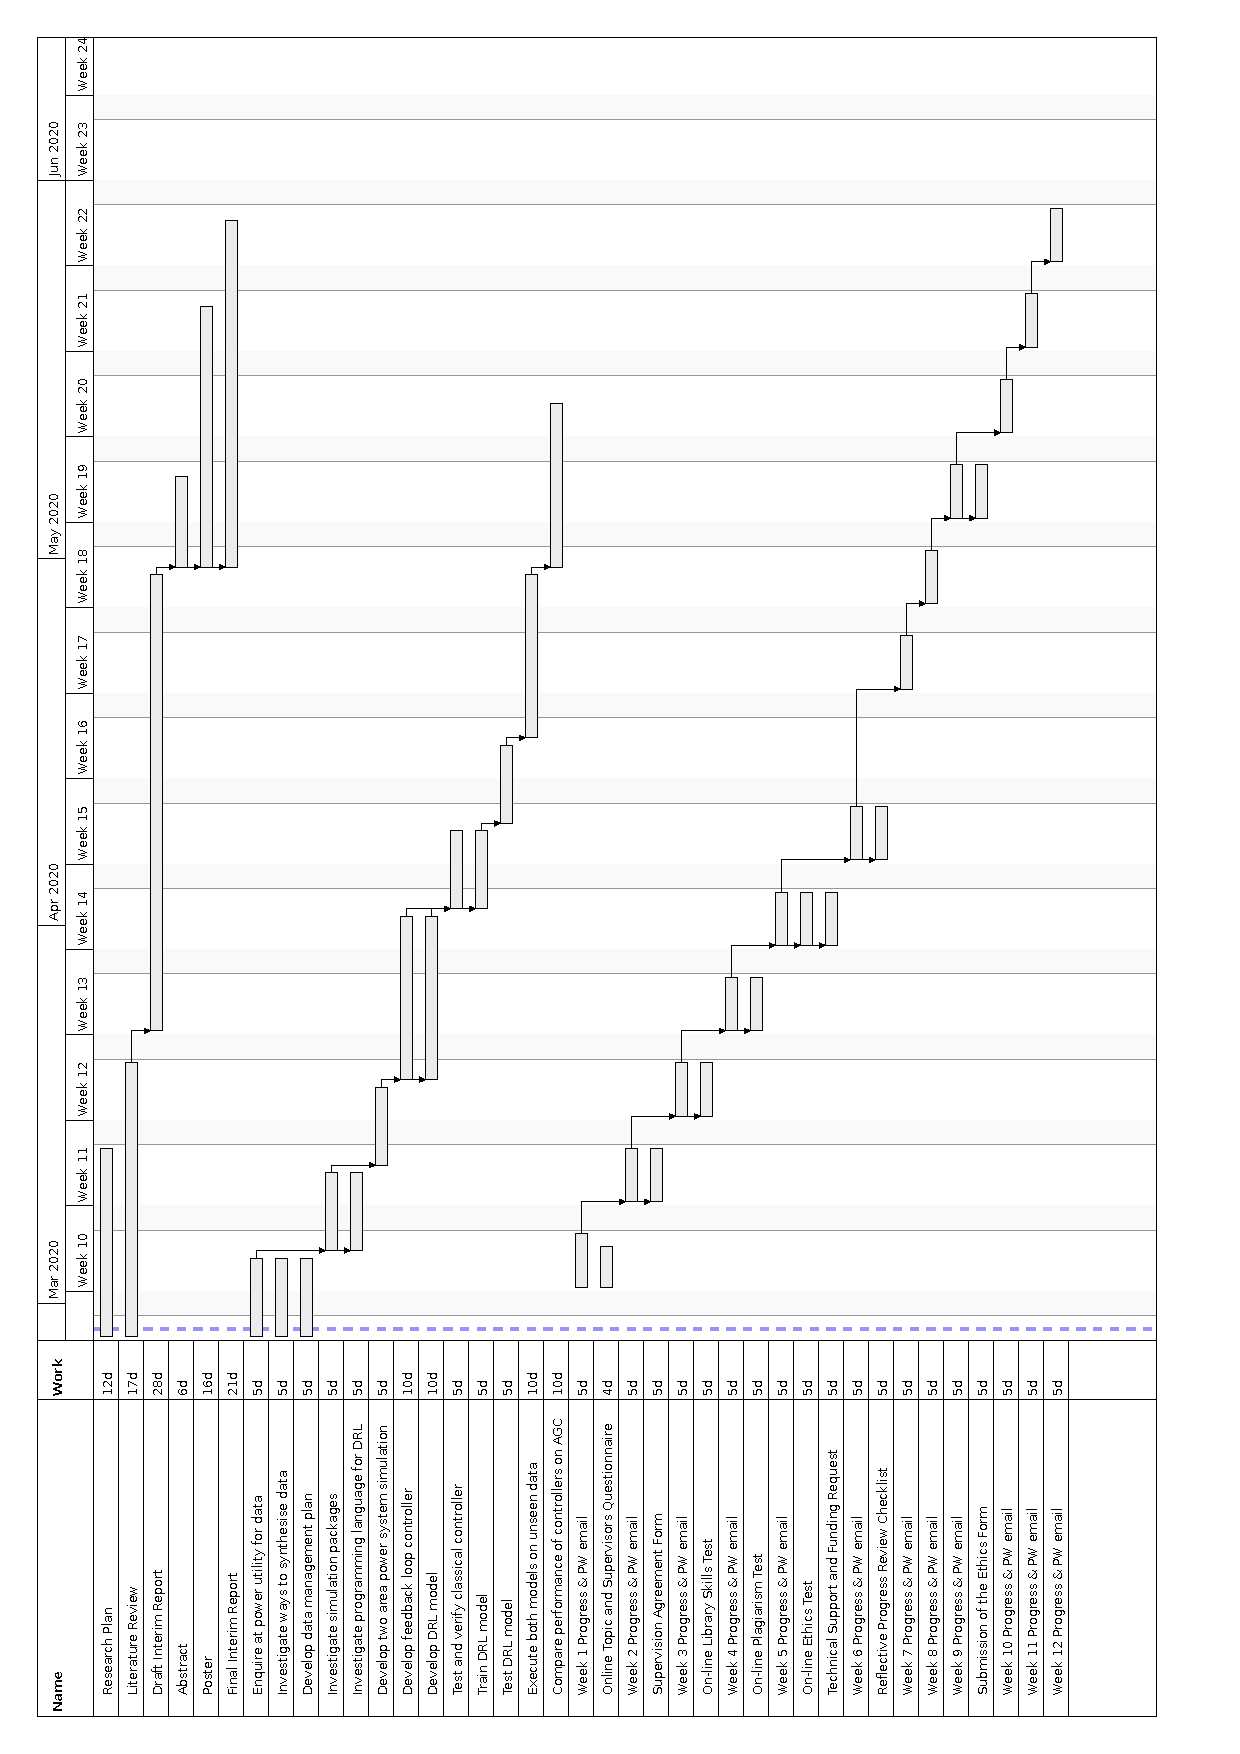
\includegraphics[scale=0.62]{./project_plan/project_plan}
\end{figure}

\clearpage

%------------------------------------
% Resources
%------------------------------------
\section{Resources}

The main research objectives, at a minimum, will require a computer with a Linux operating system, RAM, and a Graphics Processing Unit (GPU). The exact specifications of these computational resources are not yet known, and will be dependent on the size of the datasets, and the amount of computation required to optimise the the DRL agent's cost function. Currently, access has been provided to an Intel Quad Core 3.2$\si{\giga\hertz}$ i5 CPU machine with 8GB of RAM, Nvidia GTX960 GPU, and Ubuntu operating system. Most likely these resources will suffice, however, in the event that greater computational power is needed, access to a high end virtualised Amazon Web Services (AWS) system set up to conduct DRL research will be required. Currently, such an instance has been provisioned on an existing AWS account and is currently deactivated to avoid cost. Using such a system can be expensive (1 hour of compute is approximately 20AUD), however, AWS will often supply student research with monetary credit.\\



%------------------------------------
%Bibliography
%------------------------------------
\bibliographystyle{unsrt}
\bibliography{./bib/my_bib}

\end{document}